\chapter{Конструкторская часть}

В данном разделе будут разарботаны алгоритмы решения задачи коммивояжера: полный
перебор и муравьиный алгоритм, также описана структура программы.

\section{Реализация алгоритмов}
На рисунках \ref{img:brute1} -- \ref{img:rand} представлена схема 
алгоритма метода полного перебора.

\begin{figure}[h]
    \centering
    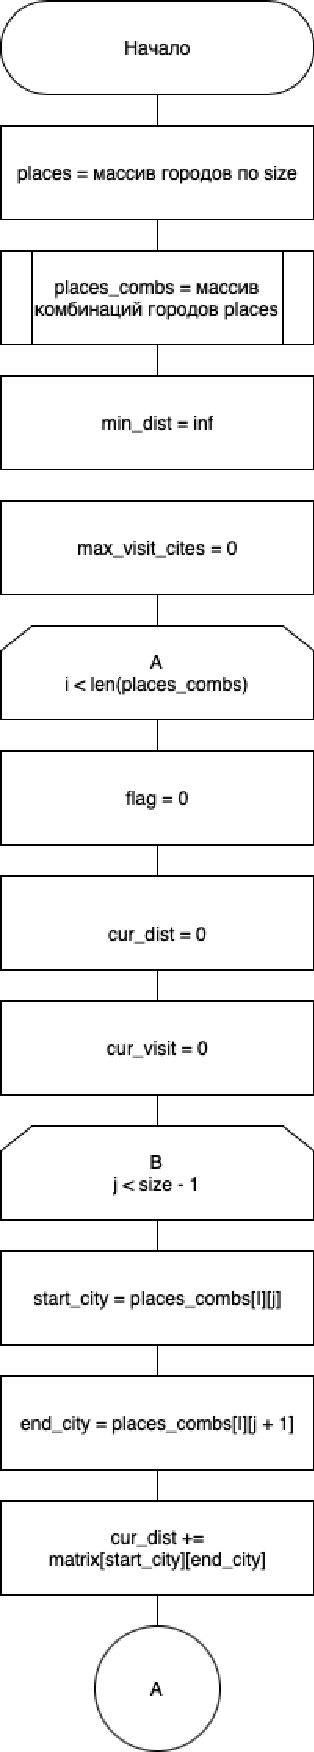
\includegraphics[width=0.25\linewidth]{img/full_comb1.pdf}
    \caption{Схема алгоритма полного перебора}
    \label{img:brute1}
\end{figure}
\noindent

\begin{figure}[h]
    \centering
    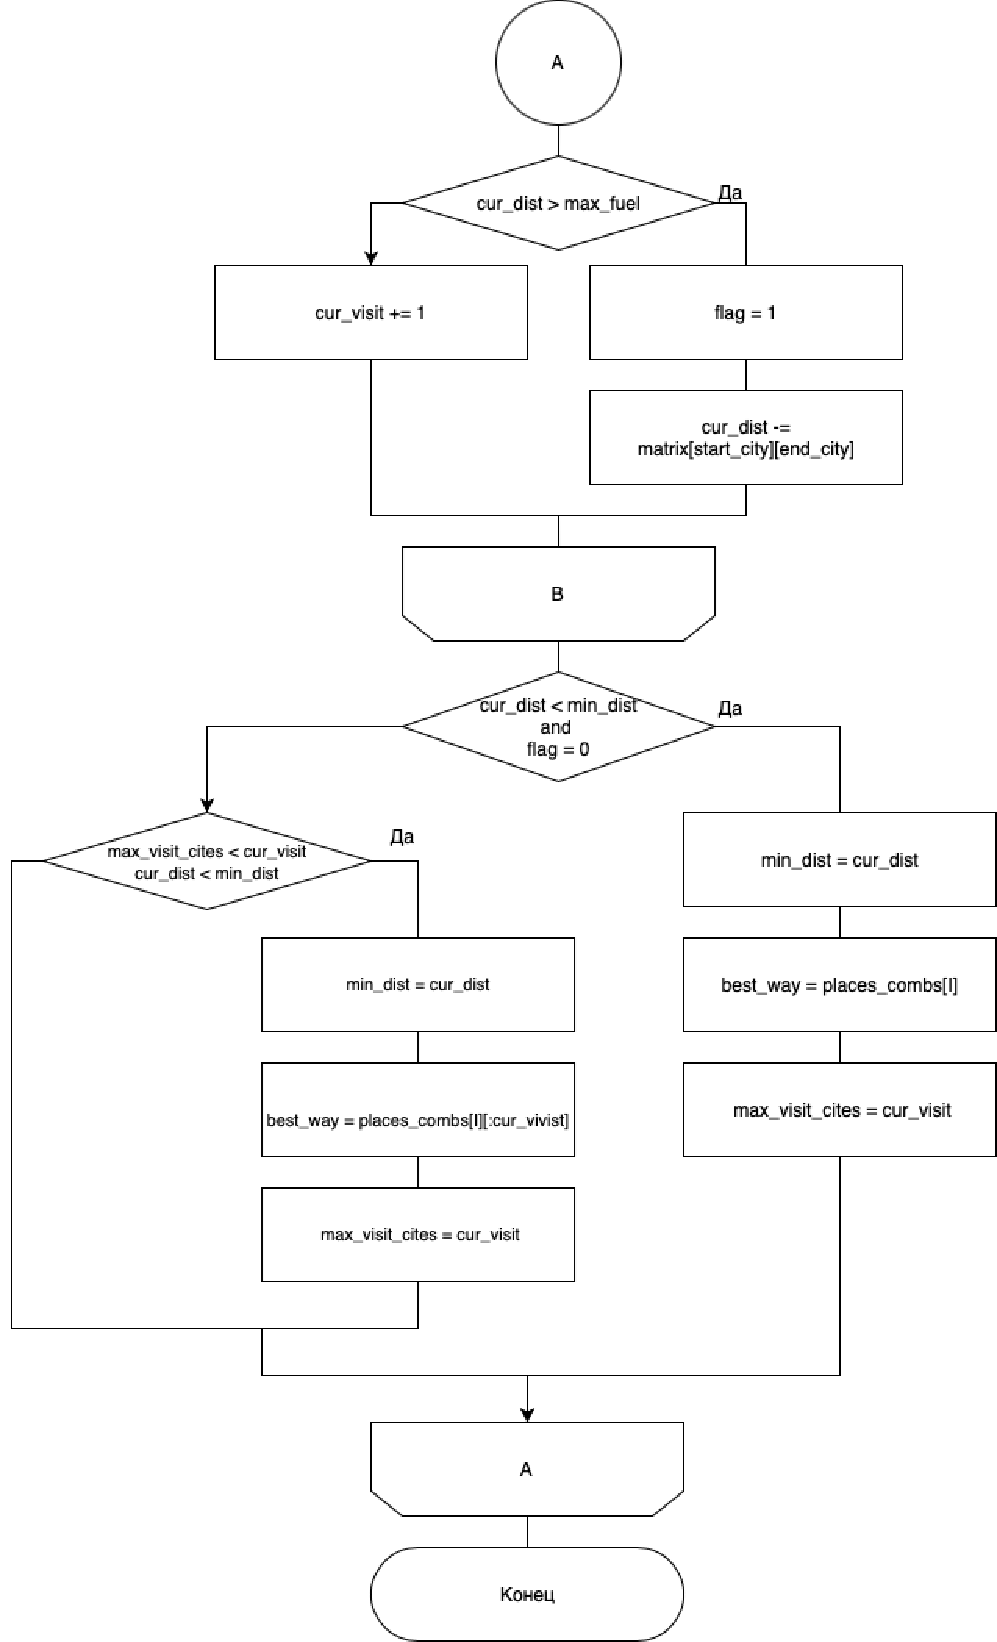
\includegraphics[width=0.80\linewidth]{img/full_comb2.pdf}
    \caption{Схема алгоритма полного перебора}
    \label{img:brute2}
\end{figure}
\noindent

\begin{figure}[h]
    \centering
    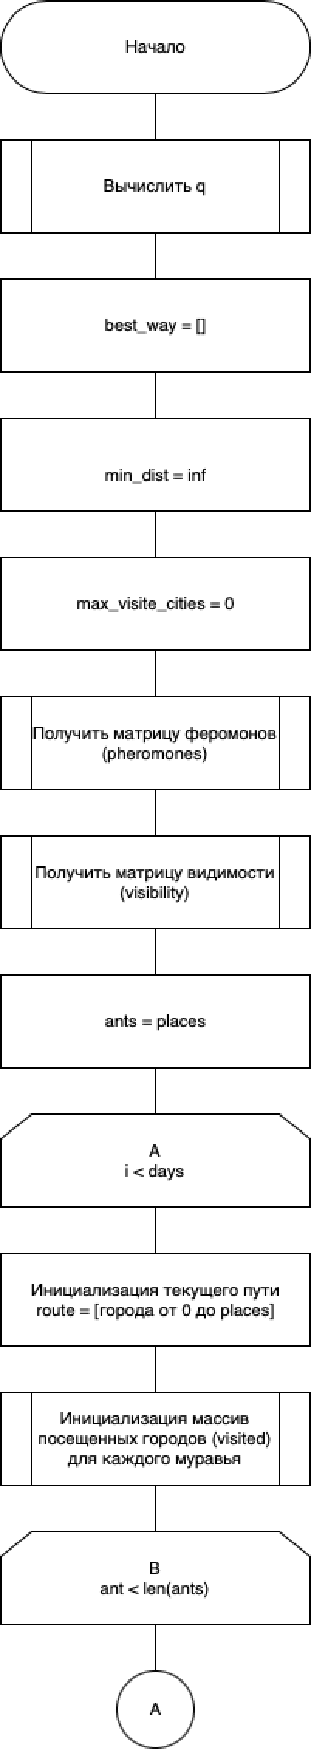
\includegraphics[width=0.25\linewidth]{img/ant_alg_part1.pdf}
    \caption{Схема муравьиного алгоритма}
    \label{img:brute2}
\end{figure}
\noindent


\begin{figure}[h]
    \centering
    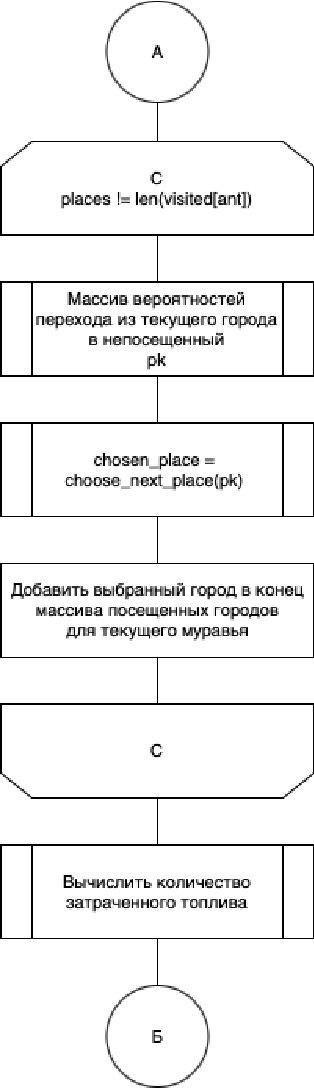
\includegraphics[width=0.30\linewidth]{img/ant_alg_part2.pdf}
    \caption{Схема муравьиного алгоритма}
    \label{img:brute2}
\end{figure}
\noindent

\begin{figure}[h]
    \centering
    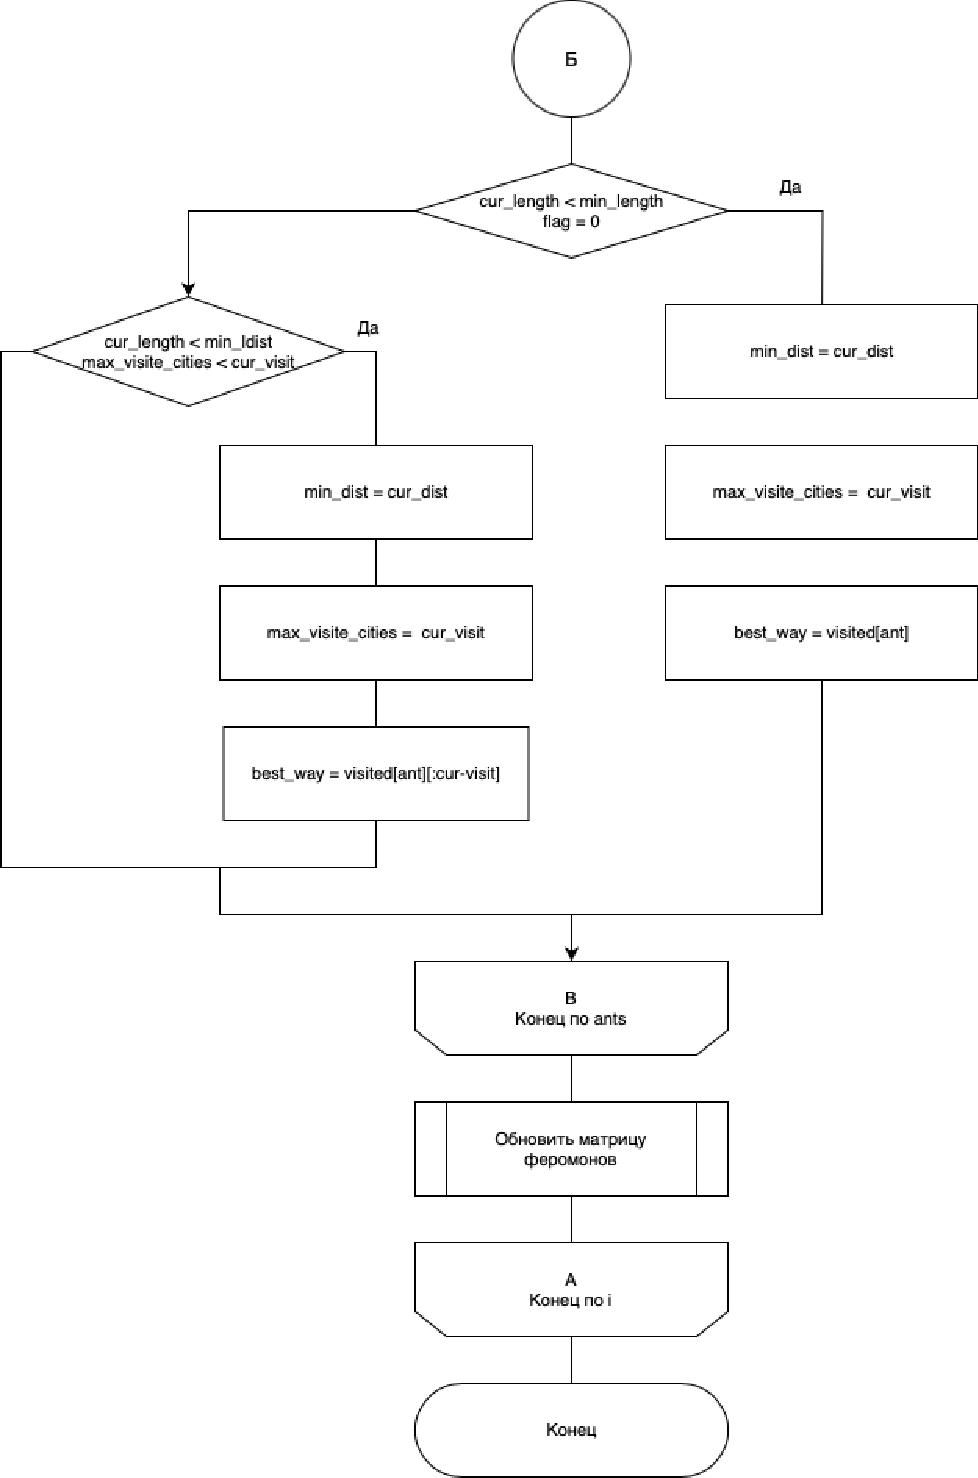
\includegraphics[width=0.65\linewidth]{img/ant_alg_part3.pdf}
    \caption{Схема муравьиного алгоритма}
    \label{img:brute3}
\end{figure}
\noindent

\begin{figure}[h]
    \centering
    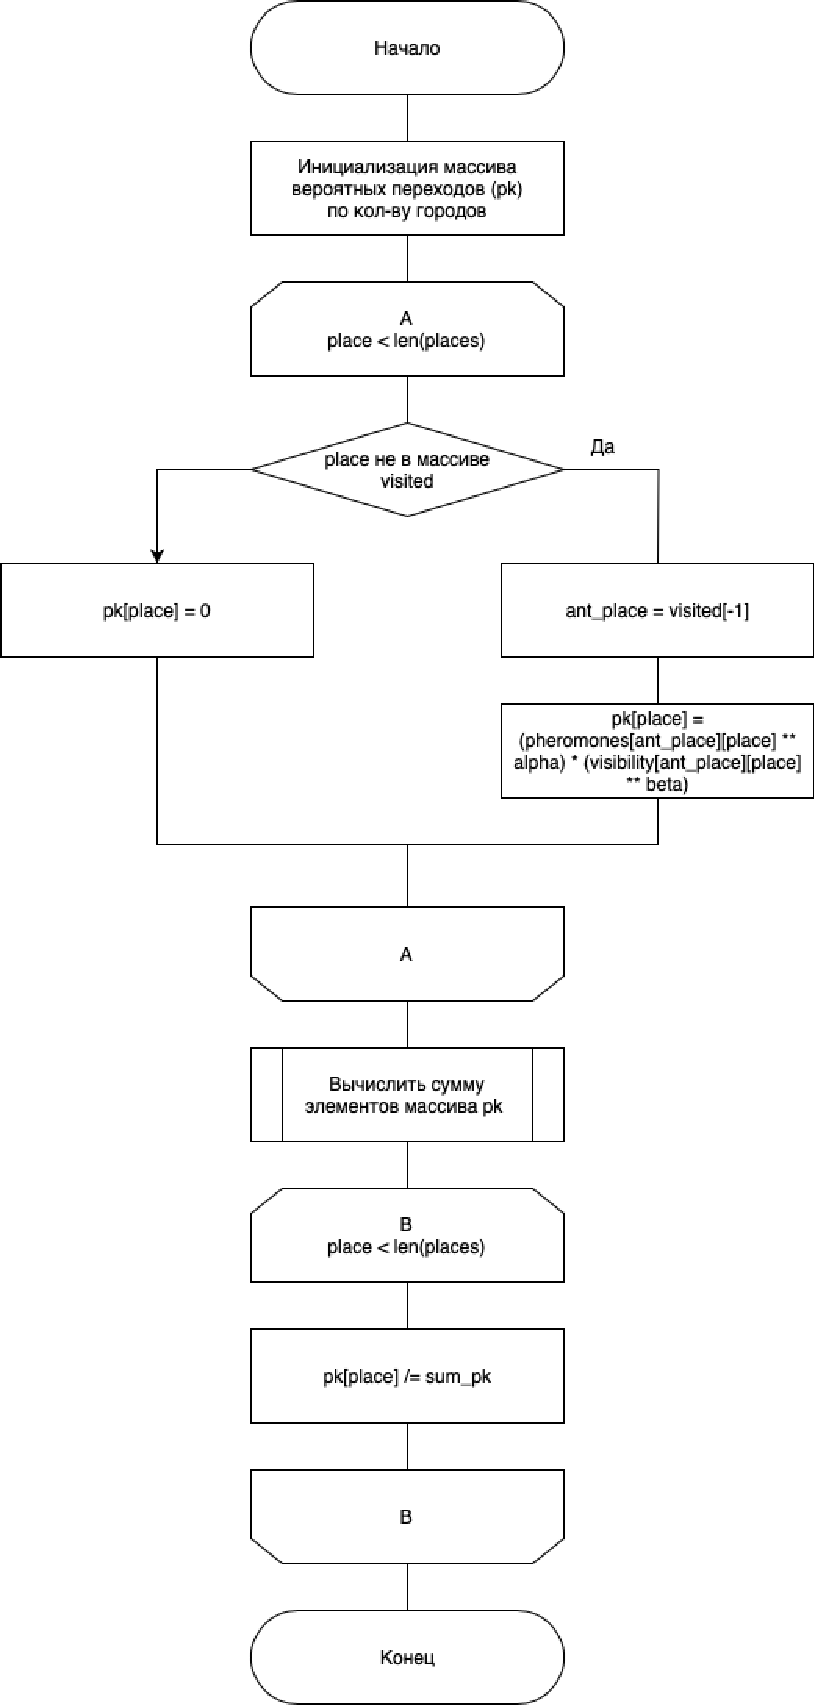
\includegraphics[width=0.60\linewidth]{img/find.pdf}
    \caption{Схема алгоритма нахождения массива вероятностных переходов в непосещенные города}
    \label{img:find}
\end{figure}
\noindent

\begin{figure}[h]
    \centering
    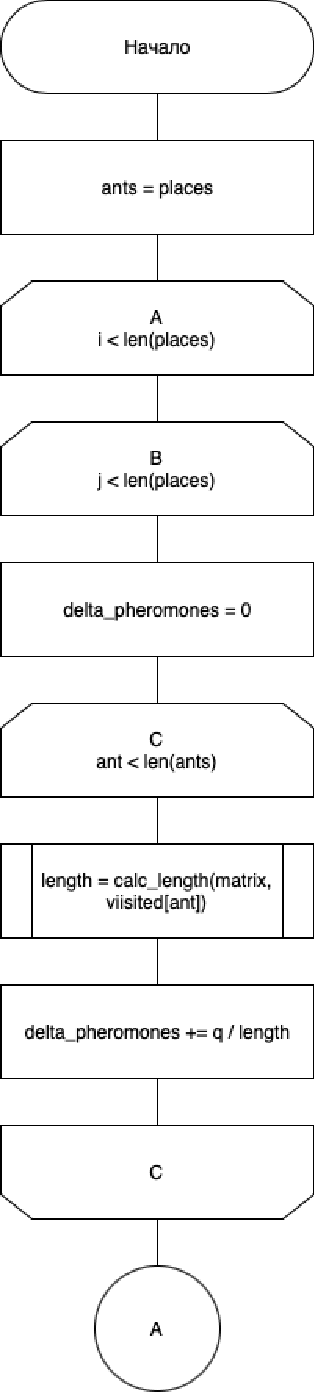
\includegraphics[width=0.30\linewidth]{img/pheromon1.pdf}
    \caption{Схема алгоритма обновления матрицы феромонов}
    \label{img:pheromon1}
\end{figure}
\noindent


\begin{figure}[h]
    \centering
    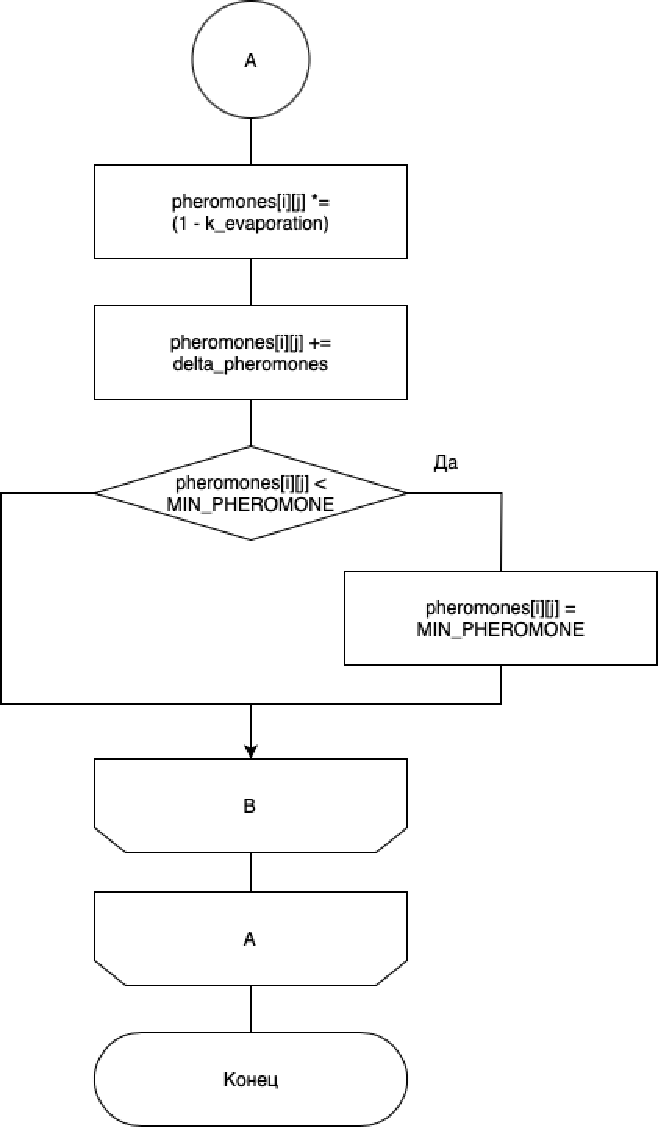
\includegraphics[width=0.55\linewidth]{img/pheromon2.pdf}
    \caption{Схема алгоритма обновления матрицы феромонов}
    \label{img:pheromon2}
\end{figure}
\noindent

\begin{figure}[h]
    \centering
    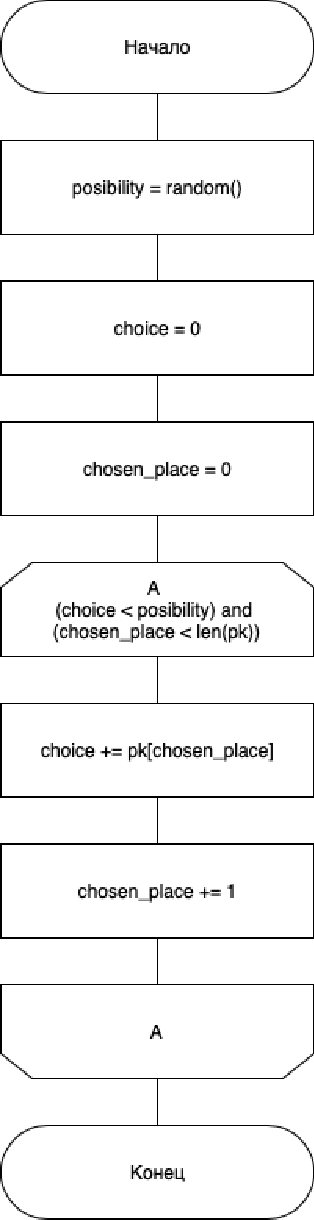
\includegraphics[width=0.25\linewidth]{img/rand.pdf}
    \caption{Схема алгоритма нахождения следующего города на основании рандома}
    \label{img:rand}
\end{figure}
\noindent

\clearpage
\section{Структура разрабатываемого программного обеспечения}

Для реализации разрабатываемого программного обеспечения будет использоваться
метод структурного программирования. Каждый из алгоритмов будет представлен
отдельной функцией, при необходимости будут выделены подпрограммы для каждой из
них. Также будут реализованы функции для ввода-вывода и функция, вызывающая все
подпрограммы для связности и полноценности программы.

\section*{Вывод}

В данном разделе были разработаны алгоритмы решения задачи коммивояжера, также была
описана структура разрабатываемого программного обеспечения.
